
\section{preliminaries}\label{sec:preliminaries}

\subsection{Lattices}\label{subsec:lattices}
This section contains the definitions and theorems of lattices, complete lattices, and partial orders.
These definitions are necessary to understand the theory behind abstract interpretation.\cite{nielson_formal_2019}

\begin{definition}
    A \textit{partial order} $(S, \sqsubseteq)$ is set $S$ equipped with a binary relation $\sqsubseteq$ that is reflexive, transitive and antisymmetric.
\end{definition}


For $X \sqsubseteq S$ and $y \in S$ we take


\begin{equation*}
    X \sqsubseteq y \iff \forall x \in X : x \sqsubseteq y,
\end{equation*}


and analogous for $y \sqsubseteq X$.


\begin{definition}
    A \textit{complete lattice} $(S, \sqsubseteq, \sqcup, \sqcap)$ is a partial order $(S, \sqsubseteq)$ in which for all $X \subseteq S:$ $\bigsqcup X$ and $\bigsqcap X$ are defined,
        \begin{equation*}
            X \sqsubseteq \bigsqcup X \land \forall y \in S : X \sqsubseteq y \implies \bigsqcup X \sqsubseteq y,
        \end{equation*}
        and
        \begin{equation*}
            \bigsqcap X \sqsubseteq X \land \forall y \in S : y \sqsubseteq X \implies y \sqsubseteq \bigsqcap X.
        \end{equation*}
\end{definition}


As a shorthand we take $x \sqcup y = \bigsqcup \{x, y\}$ and $x \sqcap y = \bigsqcap \{x, y\}$.


\begin{definition}
    A \textit{lattice} $(S, \sqsubseteq, \sqcup, \sqcap)$ is a partial order $(S, \sqsubseteq)$ in which for all $x,y \in S:$ $x \sqcup y$ and $x \sqcap y$ are defined,
        \begin{equation*}
            \{x, y\} \sqsubseteq x \sqcup y \land \forall z \in S : \{x, y\} \sqsubseteq z \implies x \sqcup y \sqsubseteq z,
        \end{equation*}
        and
        \begin{equation*}
            x \sqcap y \sqsubseteq \{x, y\} \land \forall z \in S : z \sqsubseteq \{x, y\} \implies z \sqsubseteq x \sqcap y.
        \end{equation*}
\end{definition}


\begin{theorem}\label{thm:kleene_finite}
    In a complete lattice $L$ with finite height, every monotone function $f : L \rightarrow L$ has a unique fixed point
    \begin{equation*}
        lfp(f) = \bigsqcup\{f^n(\perp) \mid n \in \mathbb{N}\}
    \end{equation*}.
\end{theorem}


\begin{theorem}\label{thm:kleene_scott}
    In a complete lattice $L$, every Scott-continuous function $f : L \rightarrow L$ has a unique fixed point $lfp(f)$.
\end{theorem}


\begin{theorem}
    If $L_1, L_2, \dots, L_n$ are complete lattices, the so is the product:
    \begin{equation*}
        L_1 \times L_2 \times \dots L_n = \{(x_1, x_2, \dots x_n) \mid x_i \in L_i\}
    \end{equation*}

    where the order $\sqsubseteq$ is defined component-wise:

    \begin{align*}
        \begin{split}
        (x_1, x_2, \dots, x_n) &\sqsubseteq (x_1', x_2', \dots, x_n') \\
        \iff
        \forall i &= 1, 2, \dots n : x_i \sqsubseteq x_i'
        \end{split}
    \end{align*}
\end{theorem}

\begin{theorem}
    If $A$ is a set and $L$ a complete lattice, then $L^A$ is a complete lattice when
    \begin{equation}
        f \sqsubseteq g \iff \forall a \in A : f(a) \sqsubseteq g(a) \text{ where } f,g \in L^A.\label{eq:equation-complete-lattice-theorem}
    \end{equation}

\end{theorem}

\todo[inline]{
    Casper says:
    The four theorems above should have a source.
}

\subsection{Abstract Interpretation}\label{subsec:abstract-interpretation}

\begin{theorem}\label{thm:galoispre}
    For $\gamma : L_1 \rightarrow L_2$ where $L_1$ and $L_2$ are complete lattices there exist a function $\alpha : L_2 \rightarrow L_1$ such that $\alpha$ and $\gamma$ forms a Galois connection if $\gamma\left(\bigsqcap B\right) = \bigsqcap_{b \in B}\gamma(b)$ for every $B \subseteq L_1$.
\end{theorem}

\subsection{Converting Code Program Graph}\label{subsec:converting-code-program-graph}
This section will briefly cover how the program graph is created.
Creating a program graph from the code is already a proven concept.
Therefore, this paper will not delve into the details but inform the reader.
The book used to show that the concept of creating a program graph from code is a proven concept~\cite[see][chap 2.2]{nielson_formal_2019}.
A program graph consists of a finite set of nodes, initial and final nodes, actions, and edges.

These directed edges represent the program's flow, and the nodes represent its state.
The edges' actions are the atomic operations that the program can perform.
The initial node is the program's starting point, and the final node is the program's end.
We denote the program graph as $edges(q_{\circ} \rightsquigarrow q_{\bullet})\llbracket I \rrbracket$ where $q_{\circ}$ is the initial node, $q_{\bullet}$ is the final node, and $I$ is the instruction.

The program graph is created by parsing the code and creating nodes and edges that represent the flow of the code. This process, while it may sound complex, is relatively straightforward. For instance, if the code is only an assignment of a variable, there will be a node for the initial state before the variable is assigned, a node for the final state after the variable is assigned, and an edge between them that represents the action of the assignment. This is written as the following equation:
$edges(q_{\circ} \rightsquigarrow q_{\bullet})\llbracket x:=a \rrbracket = \{(q_{\circ}, x:=a, q_{\bullet})\}$
$q_{\circ}$ is the initial node, $q_{\bullet}$ is the final node, and $x:=a$ is the assignment. This creates a set that represents the program graph, which can be seen in \autoref{fig:tikz-program-graph-assignment}. This is a simple example, and the program graph can be more complex depending on the code, but the concept is the same. Further examples can be found in~\cite[Figure 2.6]{nielson_formal_2019}.

\begin{figure}[htb!]
    \center
    \begin{figure}[htb!]
    \center
    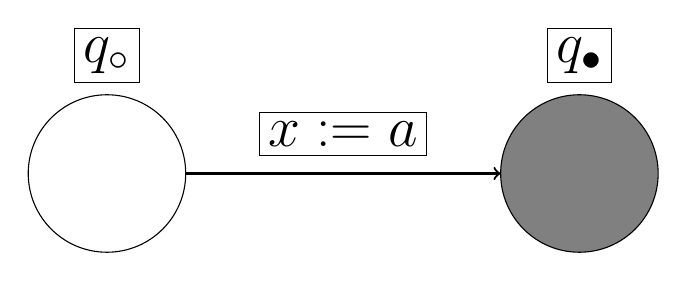
\begin{tikzpicture}
        \filldraw[fill=white, draw=black] (2,2) circle (1cm);
        \filldraw[fill=gray, draw=black] (8,2) circle (1cm);
        \node [draw] at (2,3.5) {\huge $q_{\circ}$};
        \node [draw] at (8,3.5) {\huge $q_{\bullet}$};
        \node [draw] at (5, 2.5) {\huge $x:=a$};
        \draw [thick, ->](3, 2) -- (7, 2);
    \end{tikzpicture}
    \caption{An example that shows a program graph of an assignment}
    \label{fig:tikz-program-graph-assignment}
\end{figure}
    \caption{An example that shows a program graph of an assignment}
    \label{fig:tikz-program-graph-assignment}
\end{figure}

We later describe the abstract syntax; \autoref{fig:abstract-syntax-instructions} describes the instructions the abstract syntax will contain.
There is no control structure in the abstract syntax, like if-statements and loops or sequences of instructions.
This is because the abstract syntax is simplified to make understanding the theory behind abstract interpretation easier.
This is all handled in the program graph, where the control structure is represented as edges in the program graph.

\begin{figure}
    \center
    \begin{tabular}{r l}
        $I \Coloneqq$ & $skip \mid v_a \coloneqq e \mid v_a \coloneqq ? \mid C_{sql} \mid b$
    \end{tabular}
    \caption{Abstract Syntax for Instructions}
    \label{fig:abstract-syntax-instructions}
\end{figure}

If-statements and loops are still used as boolean expressions in edges, used like guards in the program graph.
We can make equations for the edges of the program graph, where $b$ is a Boolean expression, and $S$ is a set of states done in the control structure.

For an if-statement `if b then S1 else S2`:
$edges(q_{\circ} \rightsquigarrow q_{\bullet})\llbracket \text{if } b \text{ then } S_1 \text{ else } S_2 \rrbracket = \text{let } q_{cond}, q_{if}, q_{else}, q_{merge}$ be new nodes.
\begin{align}
    S_{cond} &= edges(q_\circ \rightsquigarrow q_{if})\llbracket b \rrbracket \cup edges(q_\circ \rightsquigarrow q_{else})\llbracket \neg b \rrbracket \\
    S_{if} &= edges(q_{if} \rightsquigarrow q_{if_{out}})\llbracket S_1 \rrbracket \\
    S_{else} &= edges(q_{else} \rightsquigarrow q_{else_{out}})\llbracket S_2 \rrbracket \\
    S_{merge} &= edges(q_{if_{out}} \rightsquigarrow q_{\bullet}) \cup edges(q_{else_{out}} \rightsquigarrow q_{\bullet}) \\
    &\text{in } S_{cond} \cup S_{if_{in}} \cup S_{else_{in}} \cup S_{merge}
\end{align}

For a while loop `while b do I`:
$edges(q_{\circ} \rightsquigarrow q_{\bullet})\llbracket \text{while } b \text{ do } I \rrbracket = \text{let } q_{loop}$ be a new node.
\begin{align}
    S_{circ} &= edges(q_\circ \rightsquigarrow q_{loop}) \llbracket b \rrbracket \\
    S_{stop} &= edges(q_{\circ} \rightsquigarrow q_{\bullet})\llbracket \neg b \rrbracket \\
    S_{loop} &= edges(q_{loop} \rightsquigarrow q_{circ})\llbracket I \rrbracket \\
    &\text{in } S_{circ} \cup S_{stop} \cup S_{loop}
\end{align}

In \autoref{fig:tikz-program-graph-loop} and \autoref{fig:tikz-program-graph-if}, we see examples of how a loop and an if-statement are represented in a program graph.

\begin{figure}[htb!]
    \center
    \begin{tikzpicture}
    \tikzstyle{arrow} = [thick,->,>=stealth]
    \node [circle, draw] (start) at (0,0){};
    \node [circle, draw, fill=black] (end) at (0,-2.3){};
    \node (a) [cloud,  cloud puffs=9.4, minimum width=1cm, draw, right=2cm of start, shift={($(start.south)+(0.2,-1cm)$)}] {$I_2$};
    \node (b) [cloud,  cloud puffs=9.4, minimum width=1cm, draw, left=2cm of start, shift={($(start.south)+(-0.2,-1cm)$)}] {$I_1$};

    \draw[arrow, ->] (start) to node[below,xshift=6, yshift=10] {$\neg b$} (a);
    \draw[arrow, ->] (start) to node[below,xshift=-4, yshift=10] {$b$} (b);
    \draw[arrow, ->] (a) to node[below,scale=.7] {} (end);
    \draw[arrow, ->] (b) to node[below,scale=.7] {} (end);
\end{tikzpicture}
    \caption{An example that shows a program graph of an if-statement}
    \label{fig:tikz-program-graph-if}
\end{figure}

\begin{figure}[htb!]
    \center
    \begin{tikzpicture}
    \tikzstyle{arrow} = [thick,->,>=stealth]
    \node (a) [cloud,  cloud puffs=9.4, minimum width=1cm, draw] {S};
    \node [circle, draw, above=of a] (start) {};
    \node [circle, draw, fill=black, below=of a] (end) {};

    \draw[arrow, ->] ([shift={(0.0,0.045)}]a.east) to[bend right] node[below,scale=.7] {} (start);
    \draw[arrow, ->] (start) -- node[right,scale=.70,xshift=-15]{b} (a);
    \draw[arrow, ->] (start) to[bend right=55] node[right,scale=.70,xshift=-20]{$\neg b$} (end);
\end{tikzpicture}
    \caption{An example that shows a program graph of a loop}
    \label{fig:tikz-program-graph-loop}
\end{figure}

In the abstract syntax, we will not have formulated sequences of $I_0, I_1, I_2, \dots, I_n$ as in the program graph, but rather as a set of states $S$, where we at the end go back to the initial state, as shown in \autoref{fig:tikz-composition-graph}.

We can make equations for the edges of the composition graph, where $I_1$ and $I_2$ are instructions:
$edges(q_{\circ} \rightsquigarrow q_{\bullet})\llbracket I_1 ; I_2 \rrbracket = $ let $q$ be a new node.
\begin{align}
    S_1 &= edges(q_{\circ} \rightsquigarrow q)\llbracket I_1 \rrbracket \\
    S_2 &= edges(q \rightsquigarrow q_{\bullet})\llbracket I_2 \rrbracket \\
    &\text{in } S_1 \cup S_2
\end{align}

\begin{figure}
    \center
    \begin{tikzpicture}
    \tikzstyle{arrow} = [thick,->,>=stealth]
    \node [circle, draw] (start) at (0,0){};
    \node (a) [cloud,  cloud puffs=9.4, minimum width=1cm, draw, shift={($(start.east)+(1.5,0)$)}] {$P_1$};
    \node [circle, draw, shift={($(a.east)+(1.5,0)$)}] (b) {};
    \node (c) [cloud,  cloud puffs=9.4, minimum width=1cm, draw, shift={($(b.east)+(1.5,0)$)}] {$P_2$};
    \node [circle, draw, shift={($(c.east)+(1.5,0)$)}, fill=black] (end) {};

    \draw[arrow, ->] (start) to node[above,scale=.7] {} (a);
    \draw[arrow, ->] (a) to node[above,scale=.7] {} (b);
    \draw[arrow, ->] (b) to node[above,scale=.7] {} (c);
    \draw[arrow, ->] (c) to node[above,scale=.7] {} (end);
\end{tikzpicture}

    \caption{An example that shows a composition graph}
    \label{fig:tikz-composition-graph}
\end{figure}
